\documentclass[]{llncs}

%% Use the options 1p,twocolumn; 3p; 3p,twocolumn; 5p; or 5p,twocolumn
%% for a journal layout:
%% \documentclass[final,1p,times]{elsarticle}
%% \documentclass[final,1p,times,twocolumn]{elsarticle}
%% \documentclass[final,3p,times]{elsarticle}
%% \documentclass[final,3p,times,twocolumn]{elsarticle}
%% \documentclass[final,5p,times]{elsarticle}
%% \documentclass[final,5p,times,twocolumn]{elsarticle}

%% For including figures, graphicx.sty has been loaded in
%% elsarticle.cls. If you prefer to use the old commands
%% please give \usepackage{epsfig}

%% The amssymb package provides various useful mathematical symbols
\usepackage{amssymb}
%% The amsthm package provides extended theorem environments
%\usepackage{amsthm}
\usepackage{amsmath}

%% for url reference
\usepackage{hyperref}
\usepackage{graphicx}

\usepackage{float}

%% The lineno packages adds line numbers. Start line numbering with
%% \begin{linenumbers}, end it with \end{linenumbers}. Or switch it on
%% for the whole article with \linenumbers.
%% \usepackage{lineno}
\def\infinity{\rotatebox{90}{8}}


\begin{document}

%\begin{frontmatter}

%% Title, authors and addresses

%% use the tnoteref command within \title for footnotes;
%% use the tnotetext command for theassociated footnote;
%% use the fnref command within \author or \address for footnotes;
%% use the fntext command for theassociated footnote;
%% use the corref command within \author for corresponding author footnotes;
%% use the cortext command for theassociated footnote;
%% use the ead command for the email address,
%% and the form \ead[url] for the home page:
%% \title{Title\tnoteref{label1}}
%% \tnotetext[label1]{}
%% \author{Name\corref{cor1}\fnref{label2}}
%% \ead{email address}
%% \ead[url]{home page}
%% \fntext[label2]{}
%% \cortext[cor1]{}
%% \address{Address\fnref{label3}}
%% \fntext[label3]{}

\title{[Short Paper:] Revisiting Difficulty Control for Blockchain Systems}


%% use optional labels to link authors explicitly to addresses:
%% \author[label1,label2]{}
%% \address[label1]{}
%% \address[label2]{}

\author{Dmitry Meshkov \and Alexander Chepurnoy}
\institute{IOHK Research}

%\ead{dmitry.meshkov@iohk.io}

\maketitle

\begin{abstract}

The Bitcoin whitepaper~\cite{Nakamoto2008} states that the security of the system is guaranteed as long as honest miners control more than half of the current total computational power. The whitepaper assumes static difficulty case when it is equally hard to solve a cryptographic proof-of-work puzzle dependless on system behavior. However, a real Bitcoin network is using an adaptive difficulty adjustment mechanism.  

In this paper we introduce and analyze a new kind of attack on mining difficulty retargeting. A malicious miner is increasing his mining profits from the attack. An average time interval between blocks is increasing as a side-effect of the attack.

We propose an alternative difficulty adjustment algorithm in order to reduce an incentive to attack and also to improve stability of inter-block delays. We show that the novel approach performs better than original algorithm of Bitcoin.
	
\end{abstract}


\section{Introduction}
\label{sec:intro}

Blockchain systems have attracted a significant amount of interest after the Bitcoin whitepaper~\cite{Nakamoto2008} was published in 2008.
Bitcoin security relies on a distributed protocol based which maintains the distributed ledger. In the protocol miners are trying to find a partial hash collision in order to generate a valid block by iterating over nonce field values. That is, for a block $\mathcal{B}$~(with a random nonce included) to be valid, condition $hash(\mathcal{B}) < T$ should hold, where {\em target} parameter $T$ specifies expected hardness of a valid block generation. This hardness can be also viewed via {\em difficulty} parameter $D = \frac{1}{T}$.

Alternative systems may rely on other than finding a partial hash collision types of computational puzzles~\cite{miller2014permacoin,biryukov2017equihash}. Nevertheless, all of them assume some algorithm that changes a puzzle difficulty dynamically. These algorithms for difficulty retargeting are required in order to make an open blockchain system tolerant to participants joining and leaving the system, and also to stabilize mean latency between blocks. 
%The latter is important for several reasons:
%\begin{itemize}
%\item{With too frequent blocks it is possible for a lot of miners to have block propagation time bigger than latency between blocks. Studies show that this weakens security guarantees of a blockchain system~\cite{decker2013information,garay2015bitcoin}.}
%\item{Too big latency leads to decreasing of the network throughput~\cite{miller2016} and may be critical for high-loaded blockchain systems like Bitcoin, where blocks are already full today~\cite{armstrong2016}. Increased latency in Bitcoin network means that some transactions will never be included into blockchain. Moreover, this will lead to potentially infinite growth of unconfirmed transactions pool, preventing relaying for most of Bitcoin transactions.}
%\end{itemize}

Most of difficulty retargeting algorithms assume total computational power involved in mining process does not significantly change from epoch to epoch. 
Using more complicated retargeting algorithms with incorrect assumptions~\cite{andruiman2014} may lead to incorrect time interval between blocks even for simple case of constant hash rate. For example, it is observed that mean time between blocks in Nxt is ~2 times bigger than stated in the whitepaper~\cite{nxt}. Moreover, too ofter difficulty recalculation leads to wide distribution of time intervals between blocks and makes blockchain system unpredictable~\cite{andruiman2014}.
Varying network computational power makes this algorithms inefficient for difficulty recalculation, e.g. continuous growth of computational power leads to decreasing mean latency between blocks and average block time in Bitcoin network is ~1.07 times lower, then expected.
Noteworthy, that exponential growth of computational power, which is the situation observed in practice in accordance with Moore’s law~\cite{moore2006cramming}, is the absolutely worst case (regarding the maximal block rate) possible for Bitcoin’s difficulty retargeting algorithm~\cite{kraft2015difficulty}.
On the other side, target recalculation algorithm should be simple enough and use integer arithmetic for all computational steps, since all nodes in the peer-to-peer network have to agree absolutely on the calculated difficulty.

Original Bitcoin white-paper, states that the security of the system is guaranteed as long as there is no attacker in possession of half or more of the total computational power used to maintain the system~\cite{Nakamoto2008}.
Most of the models used in the literature to discuss double-spending attacks assume that mining difficulty is constant~\cite{??}.
However difficulty is not constant, and can be manipulated by the attacker.
The Difficulty Raising Attack, introduced in~\cite{bahack2013theoretical}, enables the attacker to discard n-depth block, for any n and any attacker hash power, with probability 1 if he is willing to wait enough time.
The fact that there is no way to determine whether a block have been computed on its declared time or not, have been used as part of other attacks~\cite{timejacking2011, artforz2011}.
In section~\ref{sec:bit} we introduce a new attack for blockchain systems which manipulates difficulty for decreasing effective hash rate, required for block generation.

Novel studies of difficulty control proposes better functions for difficulty recalculation.
For example, the paper~\cite{kraft2015difficulty} introduces target recalculation function, designed to work “perfectly” not just for constant hash rate but also if the hash rate grows exponentially (with a constant but unknown rate).
Since it's good for situation, observed in practice in Bitcoin network, there are still a lot of open questions for future research.
Is it possible to create such a function, suitable for random fluctuations in the hash rate?
Is it possible to create such a function, simple enough to use integer arithmetic for all computational steps?
Is it possible to create such a function, stable for attackers manipulations?

\textbf{TODO transition to next section}

Several parts are organizing the paper. 

\section{Bitcoin Mining}
\label{sec:bit}

The concept of Bitcoin mining was introduced in the section 4 of the Bitcoin whitepaper~\cite{Nakamoto2008} and discussed then in the papers~\cite{kraft2015difficulty, miller2014permacoin, eyal2014majority, garay2015bitcoin}. The paper~\cite{garay2015bitcoin} introduced \textit{chain quality} property for a blockchain system. The property states that if adversary holds (?) of total mining power then it could generate no more than (?) of total blocks in the long run. The result got under the assumption of static difficulty. In this paper we study what advantage an adversary could get by influencing difficulty parameter.

In Bitcoin a miner generates a block by iterating through \(nonce\) and calculating SHA-256 hash of a blocks header with the nonce value included.
For a block to be valid the hash of its header must be less than current \textit{target} \(T\): \( hash(blockheader) < T \). \textit{Difficulty} is expressed as \(\frac{1}{T}\). If output of \(hash\) function is \(\mu\) bits long then probability to generate a block by doing \(q\) requests is \(\frac{T \cdot q}{2^\mu} = \frac{q}{D \cdot 2^\mu}\). We choose a second as a time unit, and we define miner \textit{hashrate} \(R\) as \(R = \frac{q_s}{2^\mu}\), where \(q_s\) is number of queries done per time unit. The probability to generate a block within time unit then is \(\frac{R}{D}\)

%% It is shown in several works\cite{garay2015bitcoin,eyal2014majority} that an adversarial miner with \(p = \frac{R_a}{R}\) ratio of mining power could generate up to \(\mu \cdot p\) blocks in a long run. The subject of this paper is to define how an adversarial miner could achieve more than that.

Every \(M\) blocks (\(M=2016\) for Bitcoin) difficulty is recalculated as
\begin{equation}
D_{i+1}=D_i \cdot {MT\over S_m}
\end{equation}
where \(T\) is expected time interval between blocks and \(S_m\) is actual time spent to generate \(M\) blocks.
For Bitcoin observed time interval $\approx$\textit{9 min 20 sec} is less than planned \textit{T=10 min} because of continuous growth of network computational power.
Difficulty recalculation interval \(M=2016\) has been chosen in such a way to recalculate difficulty every 2 weeks.
This time interval is big enough to see computational power of the network being increased: right after target recalculation block time is close to desired 10 minutes, whereas at the end of \(epoch\) it is less than 9 minutes (see figure~\ref{fig:image}).

\begin{figure}[H]
\center{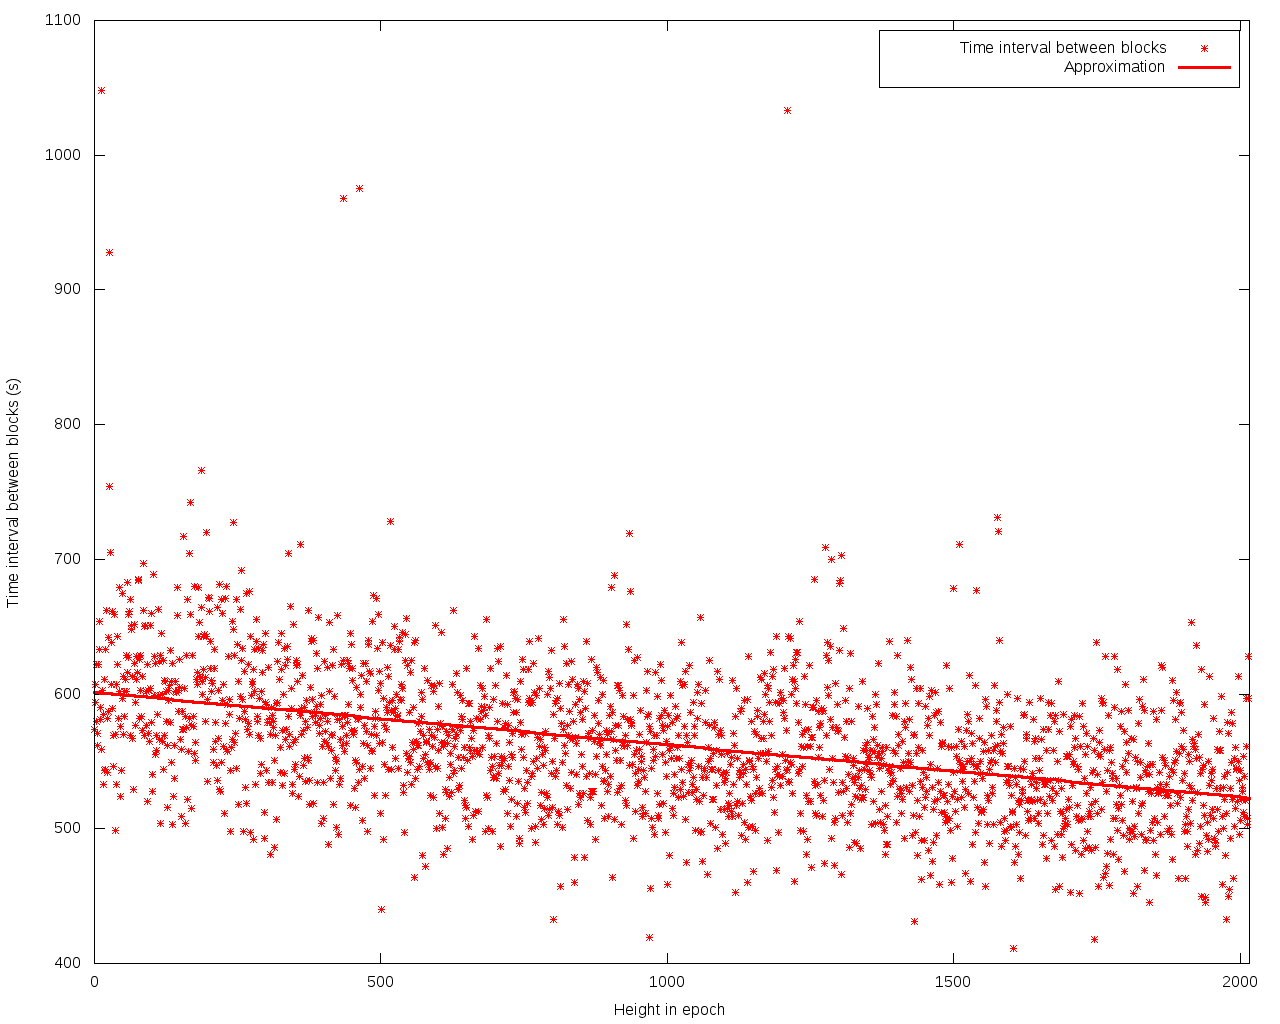
\includegraphics[scale=0.3]{interval.png}}
\caption{Average block time between difficulty recalculation}
\label{fig:image}
\end{figure}

\textbf{TODO the picture above is a mess}
\textbf{TODO transition to next section}

\section{Switching Attack}
\label{sec:attack}

We consider the following adversarial experiment involving an adversarial miner \(\mathcal{A}\):

\begin{itemize}
\item There are \(N > 1\) possible coins \(\mathcal{A}\) can contribute to. Each of them is about the same mining profitability. 
\item \(\mathcal{A}\) is mining one of the coins before a beginning of an epoch, say, epoch A. At this moment he switches to mine other coins. 
\item Without a contribution of \(\mathcal{A}\) mining power for the epoch goes down. 
\item For an epoch B next to the epoch A where \(\mathcal{A}\) left difficulty re-adjusted to a lower value. So \(\mathcal{A}\) starts mining again with a lower difficulty. 
\end{itemize}

We call this strategy a \textit{switching attack}.

To calculate adversarial profit from the attack we assume Bitcoin difficulty recalculation function and constant hash rate.

Consider the network has hash rate \(R_0\) provided by honest miners and the adversary has additional hash rate \(R_a=R_0\cdot p\) to turn it on or off.
Before epoch A the adversary mines all the time with difficulty \(D_0 = (R_0+R_a) \cdot T\) and will mine \(M\cdot R_a\over R_0+R_a\) blocks per epoch (\(M\) blocks) in average spending \(M \cdot R_a \cdot T\) computational power for them.
During the epoch B the adversary mines with difficulty \(D_1 = R_0 \cdot T\) is calculated from honest miners \(R_0\) only.
He will mine \(M\cdot R_a\over 2(R_0+R_a)\) blocks per epoch in average spending \(M\cdot T\cdot R_a\cdot R_0\over 2(R_0+R_a)\) computational power for them.
Consequently honest miner will spend \((R_0+R_a)T\) computational power per block, whereas attacker will just spend \(R_0T\) computational power per block.
The cost of computational resources invested into mining should be around the expected reward.
If \(B\) is block reward and \(C\) is hash calculation cost, the honest miner profit is
\begin{equation}
{({M\cdot R_a\over R_0+R_a})\cdot B-M\cdot R_a\cdot T\cdot C=M\cdot R_a\cdot ({B\over R_0+R_a}-TC)}
\end{equation}
per epoch.
At the same time adversarial profit is
\begin{equation}
{{M\cdot R_a \over 2\cdot (R_0+R_a)}\cdot (B - T\cdot R_0\cdot C)}
\end{equation}


Additional profit of the adversary is:
[TODO: ???]
\begin{equation}
{{B\over C} < T\cdot (R_0+2\cdot R_a)}.
\end{equation}



Remarkable, that under such an attack mean time between blocks will be
\begin{equation}
\label{eq:ati}
{T_a={T\over 2}({R_0+R_a\over R_0} + {R_0\over R_0+R_a})=T(1 + {p^2\over 2(1+p)})}
\end{equation}
which is bigger then desired time \(T\).
Please notice that we regard \(p\) as the ratio between the hash-powers of the attacker and the honest network so it changes from 0 to 1.

\textbf{TODO transition to next section}

\section{Improved Difficulty Adjustment}
\label{sec:improved}

The difficulty adjustment algorithm employed by Bitcoin works as designed: If the hash rate is constant, it yields the desired block rate. However it does not achieve the desired block rate in other situations and vulnerable to attack, described in \ref{sec:attack}.
In this section we are going to propose an alternative difficulty adjustment algorithm that works better than the Bitcoin's.

First, we state properties of an \(ideal\) difficulty update algorithm:
\begin{enumerate}
\item{It should be resistant to known types of attacks based on difficulty manipulation.}
\item{It should lead to desired block rate for random fluctuations in the hash rate.}
\item{It should be simple enough to use integer arithmetic for all computational steps.}
\end{enumerate}

Security is the most important feature of blockchain systems and should be regarded with the highest priority.
Incorrect block rate is not considered a big problem in the Bitcoin community but it may be important for more advanced applications of blockchain systems.
Implementation of the \textit{ideal} difficulty update algorithm in subclass of integer programming is desired for different platforms compatibility.
This rule is not required, because, as mentioned in \cite{kraft2015difficulty}, it is possible to include non-integer algorithm parameters as part of the block, but it provides another way of difficulty manipulating to an attacker.

In this section we are going to regard difficulty adjustment algorithm based on well-known linear least squares method\cite{lawson1974solving}. In the simpliest case of pair linear regression (\(y=kx+b)\) coefficients may be calculated as follows:

\begin{equation}
  \begin{cases}
    k= {{\overline{xy} - \overline{x}\overline{y}} \over {\overline{x^2} - \overline{x}^2}}  \\
    b= \overline{y}-k\overline{x}
  \end{cases}
\end{equation}

Note, that for accurate difficulty prediction we should use few last observed difficulties, rather than just one, as implemented in Bitcoin, but it's possible to use this algorithm right after second epoch.


We regard it as the good candidate for difficulty update algorithm, because:
\begin{enumerate}
\item{It should reduce profit of the attack, described in Section~\ref{sec:attack}. Calculations of the attacker profit are described in Section~\ref{sec:sim}}
\item{It leads to desired block rate for linear changes in the hash rate.
This means, that regarding block rate, linear algorithm is better, then Bitcoin's one, in all cases, except constant hash rate, when they lead to the same result. }
\item{It is simple enough to use integer arithmetic for all computational steps with high fidelity.}
\end{enumerate}

\section{Simulations}
\label{sec:sim}

We present simulation results that show how our method proposed in Section~\ref{sec:improved} improves over Bitcoin’s difficulty update algorithm.
We will regard \textit{difficulty} growth in this section, keeping in mind the fact, that it's closely related with network hash rate, which is usually considered in literature.

All calculations have been performed with open-sourced programs, available at Scorex project GitHub page~\cite{scorex}.

\textbf{TODO Linear?}

\subsection{Exponential Difficulty}

First, we observe exponential difficulty growth occurred in practice in Bitcoin network. As we already mentioned, exponential difficulty growth is the absolutely worst case possible for Bitcoin’s difficulty retargeting algorithm.
For simplicity we regard a situation, when hash rate growth 10\% each epoch, more complicated research of exponential difficulty growth can be found in~\cite{kraft2015difficulty}.
Figure~\ref{fig:exp} presents difficulty as the function of epoch, which is 2016 blocks in Bitcoin.

\begin{figure}[h]
\center{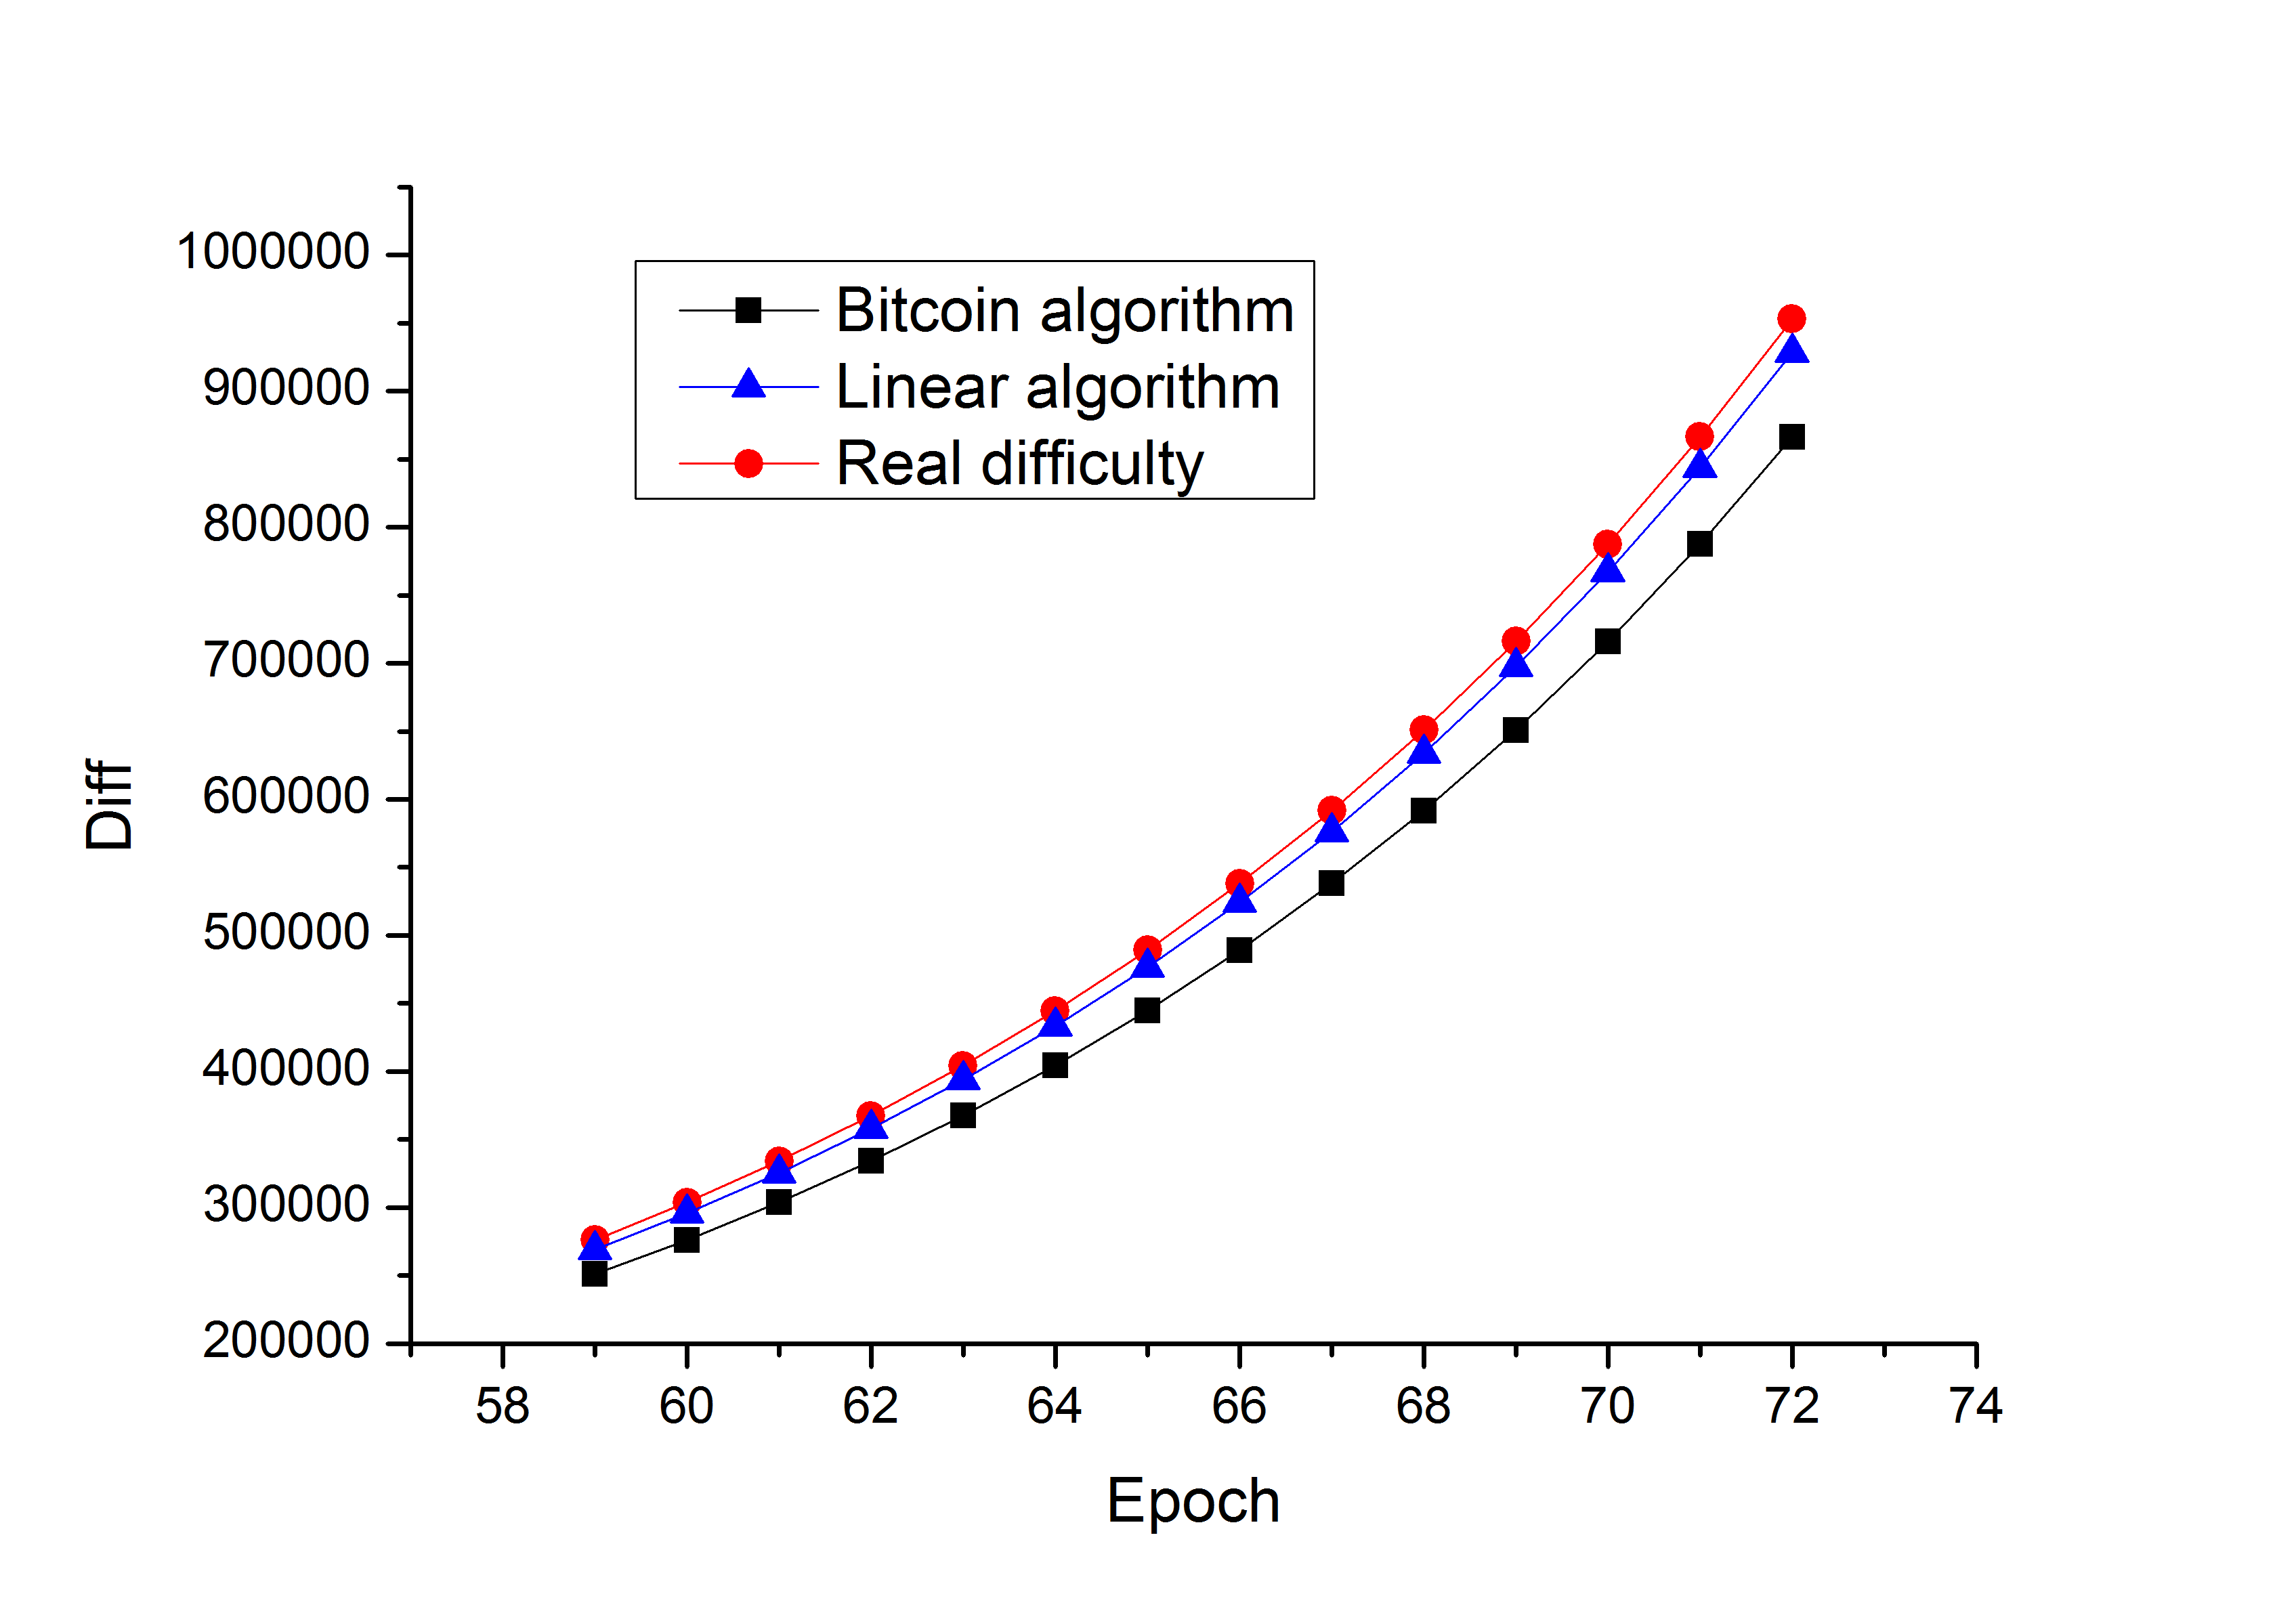
\includegraphics[scale=0.3]{exp.png}}
\caption{Real difficulty (red) and difficulties calculated from bitcoin (black) and linear (blue) algorithms in situation of exponential hash rate growth}
\label{fig:exp}
\end{figure}

Note that difficulty calculated from Bitcoin algorithm is always significantly lower than the real one.
This leads to \textit{9 min 5 sec} time interval between blocks, which is $\approx$10\% lower then desired \textit{10 min} interval.
Difficulty, calculated from Linear algorithm is also always lower, then the real one, while it's much closer to it.
Mean time interval between blocks is \textit{9 min 45 sec}, which is much closer to the desired one.

While difficulty update algorithm, proposed in~\cite{kraft2015difficulty} leads to much better results for exponential difficulty growth with a constant rate, we should note, that our algorithm is much simplier and may be implemented with integer arithmetic only.
Moreover, exponential difficulty growth is the simplification of the difficulty growth law, and it may be incorrect to expect it in some situations.

\subsection{Switching Attack}

We consider a situation described in the Section~\ref{sec:attack}: an attacker with computational power \(R_a\) (for simplicity we suppose \(R_a=0.2 \cdot R_a \) in this section) turn on and turn off his mining to manipulate difficulty and minimize computational power, expended for block mining.
Figure \ref{fig:exp} represents difficulty as the function of epcoh for this situation.

\begin{figure}[h]
\center{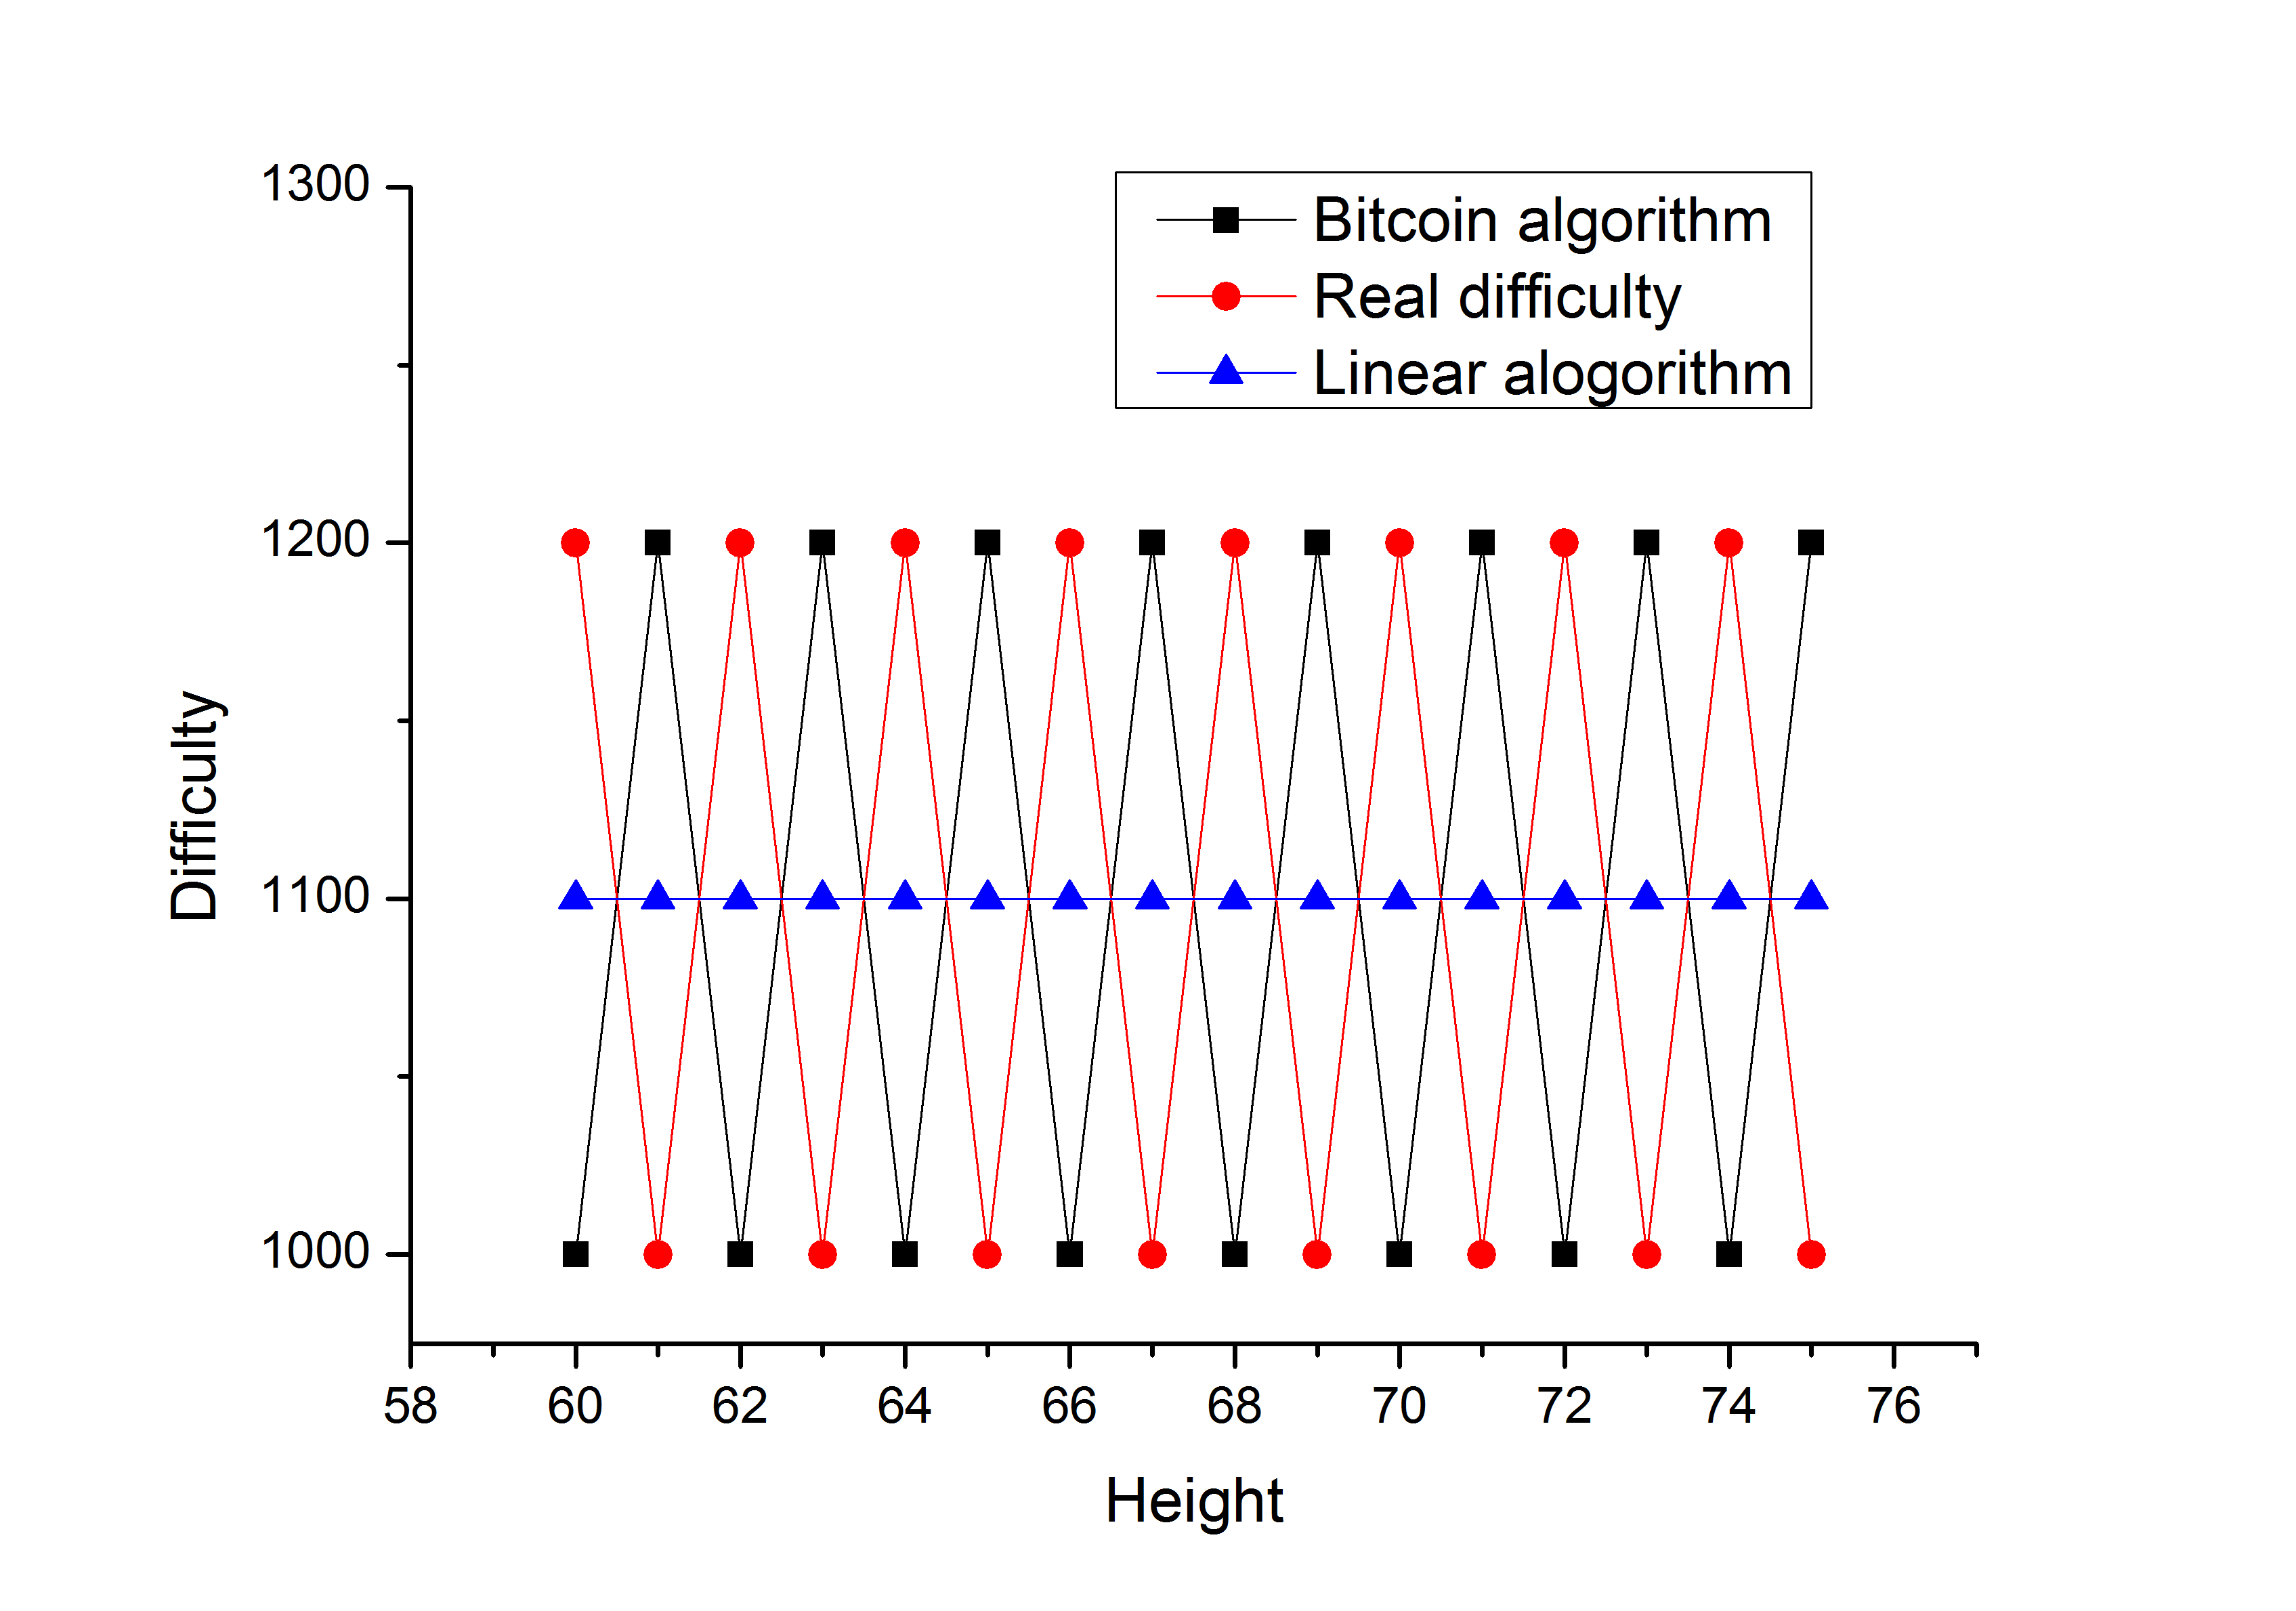
\includegraphics[scale=0.3]{attack.png}}
\caption{Real difficulty (red) and difficulties calculated from bitcoin (black) and linear (blue) algorithms in situation of attack, described in section \ref(sec:attack)}
\label{fig:attack}
\end{figure}

Note that the difficulty calculated with the Bitcoin algorithm is always in antiphase with the real one and the attacker spends his computational power only when difficulty is low.
Bitcoin difficulty update algorithm leads to \textit{10 min 10 sec} mean delay between blocks, which is in good correlation with \ref{eq:ati}.
Linear algorithm also leads to enlarged time interval between blocks \textit{10 min 5 sec}, but it's deviation from desired time is 2 times lower.
Obviously, attacker profit is also 2 times lower in situation with linear difficulty update algorithm, which may be regarded as a good result.

Thus, linear difficulty control algorithm, proposed in Section \ref{sec:improved} is better than the Bitcoin's in all situations both in terms of block rate and in terms of attacker profit.

\section{Conclusion}
\label{sec:concl}

In this paper we analyze a new kind of attacks on the blockchain based on manipulating mining difficulty.
This attack decrease computational power spent by an attacker for block mining while increasing mean time interval between blocks.
It is especially favorable in situation, when the cost of computational resources invested into mining is around the expected reward and there are enough forks to switch mining between them.

To improve the stability of block times and decrease the attacker profit, we proposed an alternative difficulty update algorithm, based on linear regression.
It was found that this algorithm is better then the Bitcoin one both in terms of block rate and in terms of attacker profit, while it's still simple enough to be computed with integer arithmetic only.

\section*{Acknowledgments}

\bibliographystyle{elsarticle-num}
\bibliography{sources.bib}


\end{document}